\documentclass[letterpaper]{IEEEtran}

\usepackage[utf8]{inputenc}
\usepackage[T1]{fontenc}
\usepackage{amsmath,amssymb}
\usepackage{graphicx}
\usepackage{booktabs}
\usepackage{multirow}
\usepackage{xcolor}
\usepackage{hyperref}
\usepackage{balance}
\usepackage{algorithm}
\usepackage{algorithmic}
\usepackage{subcaption}
\usepackage{siunitx}

% Compact lists
\usepackage{enumitem}
\setlist{nosep,leftmargin=*}

\hypersetup{
  colorlinks=true,
  linkcolor=black,
  citecolor=blue!60!black,
  urlcolor=blue!60!black,
}

\title{FLARE: A Contract-Verified Benchmark for\\
       Risk-Aware UAV Planning Under Coupled Dynamic Hazards}

\author{%
  \IEEEauthorblockN{Konstantinos~Zervakis\IEEEauthorrefmark{1}
    \and Elias~Panagiotopoulos\IEEEauthorrefmark{1}}
  \IEEEauthorblockA{\IEEEauthorrefmark{1}Athens, Greece}
}

\begin{document}

\maketitle

% ============================================================================
\begin{abstract}
We present FLARE, an open-source benchmark for UAV path planning
in disaster-response scenarios where planner decisions have
\emph{human consequences}.  Three OpenStreetMap-derived urban
scenarios---pharmaceutical delivery during wildfire, multi-casualty
urban rescue, and fire-perimeter surveillance---feature wind-driven
cellular-automaton fire, structural collapse with permanent debris,
traffic closures, and multi-POI missions with time-decaying impact scores.  A \emph{risk cost map} translates
hazard proximity into per-planner costs.
Five planners are evaluated across 450~episodes (30~seeds).
Beyond navigation success, we introduce \emph{mission scores}
that quantify medication efficacy, casualty survival, and
surveillance freshness.  These scores reveal ranking inversions:
planners that reach the goal may score lower than those that
prioritize task completion.
A contract architecture (36~invariants, 15~families) guarantees
deterministic replay and planner fairness.
All experiments are bit-identical under the same seed triple.
Code and data: \texttt{MIT license}.
\end{abstract}

\begin{IEEEkeywords}
UAV path planning, disaster response, benchmarking, dynamic environments,
fire spread, mission-impact scoring, reproducibility
\end{IEEEkeywords}

% ============================================================================
\section{Introduction}\label{sec:intro}

When a UAV delivers insulin to a fire-isolated village, every
minute of delay degrades the medication.  When it triages
fire-stranded casualties, the order and speed of visits determine
who survives.  Standard path-planning benchmarks reduce these
missions to a binary: did the agent reach the goal?  They
cannot distinguish a planner that delivers insulin in 200~steps
from one that arrives in 800---yet the patient outcomes are
vastly different.

UAVs are increasingly deployed in disaster
response~\cite{Erdelj2017,Yuan2015,Yucesoy2025,Rahim2025},
where wildfires advance under wind and buildings collapse.
Path planning algorithms must handle \emph{dynamic} obstacles
in rapidly evolving environments~\cite{Meng2025,Dradoum2025}.
Despite extensive research~\cite{Aggarwal2020,Zhao2020},
reproducible comparison under controlled dynamic conditions remains
difficult: ad-hoc scenarios, fixed obstacles, and proprietary
simulators~\cite{Henderson2018} prevent isolation of environmental
effects.  Furthermore, existing benchmarks report only navigation
success, ignoring the \emph{mission impact} of planning
decisions~\cite{Agarwal2021}.

We address these gaps with \textbf{FLARE}, a benchmark framework with
four design principles:

\begin{enumerate}
  \item \textbf{Deterministic reproducibility.}  Given the same
    $(scenario, planner, seed)$ triple, the framework produces
    bit-identical trajectories, event logs, and metrics.  A single
    root RNG, spawned per episode, drives all stochastic components.

  \item \textbf{Planner fairness.}  All planners receive identical
    observations at each step.  Dynamic obstacles evolve \emph{after}
    the agent moves, and interdictions are placed on the A*-reference
    corridor independent of which planner is under evaluation.

  \item \textbf{Hazard-coupled planning.}  Wind-driven
    fire~\cite{Alexandridis2008}, continuous risk cost maps,
    and structural collapse create a rich hazard landscape that
    differentiates planners by their risk tolerance, not just their
    replanning frequency.

  \item \textbf{Rigorous evaluation.}  We adopt the statistical
    protocol of Agarwal et al.~\cite{Agarwal2021}: interquartile mean
    (IQM) with bootstrap confidence intervals, Friedman
    tests~\cite{Demsar2006}, Cliff's delta effect sizes, and
    performance profiles~\cite{Dolan2002}.
\end{enumerate}

The framework implements a Gymnasium-compatible~\cite{Towers2025}
environment with three urban scenarios built from OpenStreetMap
data~\cite{Boeing2017}, each inspired by real Greek disaster events
(2021~Evia wildfires, 2023~Piraeus coastal fires, 2023~Evros megafire).
Five planners from three algorithmic families are evaluated:
A*~\cite{Hart1968}, Incremental~A* (inspired by
D*~Lite~\cite{Koenig2002}), APF~\cite{Khatib1986}, and two
A*-based replanning variants.

\textbf{Contributions.}
\begin{itemize}
  \item Multi-POI disaster-response missions with time-decaying
    impact scores (medication efficacy, casualty survival,
    surveillance freshness) that reveal ranking inversions
    invisible to navigation-only metrics.
  \item An open-source, contract-verified framework
    (36~invariants, 15~families) with wind-driven fire
    and per-planner risk costs.
  \item Three OSM-based urban scenarios with physically motivated
    dynamic obstacles and operationally grounded missions.
  \item A 450-episode study with rigorous statistical analysis,
    plus ablation studies isolating individual dynamics layers.
\end{itemize}

% ============================================================================
\section{Related Work}\label{sec:related}

\subsection{UAV Path Planning}

Classical UAV planners include A*~\cite{Hart1968},
D*~Lite~\cite{Koenig2002}, sampling-based methods (RRT, PRM),
and APF~\cite{Khatib1986}.  Recent surveys~\cite{Meng2025,Dradoum2025}
emphasize benchmarks under dynamic, uncertain conditions.
Risk-aware planning~\cite{Zhou2025,Melissaris2025} uses continuous
cost maps from hazard proximity; FLARE implements per-planner risk
coefficients for risk-tolerant vs.\ risk-averse comparison.

\subsection{Benchmarking and Reproducibility}

Henderson et al.~\cite{Henderson2018} showed RL results are sensitive
to seeds and evaluation methodology.
Agarwal et al.~\cite{Agarwal2021} proposed IQM with bootstrap CIs;
Dem\v{s}ar~\cite{Demsar2006} formalized Friedman/Wilcoxon tests;
Dolan and Mor\'e~\cite{Dolan2002} introduced performance profiles.
FLARE adopts all four.
Gymnasium~\cite{Towers2025} provides the standard environment API;
Bonsignorio et al.~\cite{Bonsignorio2025} argue for reproducible
robotics benchmarks---a principle central to FLARE's contracts.

\subsection{Dynamic Environments}

Alexandridis et al.~\cite{Alexandridis2008} proposed CA wildfire
models; recent work~\cite{Giannino2025,Sahila2025} confirms wind
as the dominant spread parameter.  FLARE extends this with
directional modulation and smoke diffusion.
Boeing~\cite{Boeing2017} introduced OSMnx for rasterized urban terrain.

% ============================================================================
\section{System Design}\label{sec:system}

\subsection{Overview}

FLARE is a Python framework built around a single Gymnasium
environment (\texttt{UrbanEnvV2}) with deterministic dynamics.
A benchmark runner orchestrates episodes: it resets the environment
with a seed, initializes the planner, and iterates the step loop
until termination.  The runner owns the authoritative step counter;
all components (dynamics, logger, renderer) receive it as a parameter.

The architecture follows a layered design:
\emph{(i)}~scenario configs define map, dynamics knobs, and
mission parameters;
\emph{(ii)}~the environment manages grid state, collision semantics,
and dynamics stepping;
\emph{(iii)}~planners implement a unified \texttt{PlannerBase} interface
(\texttt{plan()}, \texttt{update()}, \texttt{should\_replan()});
\emph{(iv)}~the runner enforces the step protocol and collects metrics.

\begin{algorithm}[htbp]
\caption{Episode Runner}\label{alg:runner}
\footnotesize
\begin{algorithmic}[1]
\REQUIRE scenario $s$, planner $\pi$, seed $k$
\STATE $\text{rng} \gets \text{RNG}(k)$; \ $(o, \text{mask}) \gets \text{env.reset}(s, \text{rng})$
\STATE $\pi.\text{init}(o)$; \ $t \gets 0$
\WHILE{$t < T_{\max}$ \AND \NOT done}
  \STATE $a \gets \pi.\text{act}(o, \text{mask})$ \COMMENT{mask frozen}
  \STATE $(o, r, \text{done}, \text{info}) \gets \text{env.step}(a)$
  \STATE \COMMENT{Dynamics advance \emph{after} move}
  \STATE $\text{mask} \gets \text{BlockingMask}(o)$; \ $t \gets t + 1$
\ENDWHILE
\RETURN metrics$(t, o, \text{info})$
\end{algorithmic}
\end{algorithm}

\subsection{Environment}

The environment operates on a $500 \times 500$ grid with
$\text{Discrete}(5)$ actions: four cardinal moves and STAY.
The observation includes agent position, goal, terrain, and the
current dynamic state.
Within each step, the planner sees the \emph{current} blocking mask
(frozen), dynamics advance only \emph{after} the move executes
(Algorithm~\ref{alg:runner}, lines~4--7).
Static obstacles cause hard collisions; dynamic obstacles
(fire, traffic, smoke) cause soft rejections logged via
a \texttt{RejectReason} enum.
If fire or debris \emph{reaches} the agent's cell after
the dynamics advance, the episode terminates immediately
(\textsc{fire\_caught} or \textsc{debris\_caught})---the
UAV is destroyed by the hazard it failed to evade.

\subsection{Dynamic Obstacles}\label{sec:dynamics}

Three dynamics layers operate simultaneously:

\textbf{Fire CA.}  Wildfire spread follows a cellular automaton on the
Moore neighborhood (8-connected).  Cell states transition
$\text{UNBURNED} \to \text{BURNING} \to \text{BURNED\_OUT}$.
When wind speed is zero, spread is isotropic with land-use-dependent
probabilities (urban $p{=}0.06$, forest $p{=}0.15$, road $p{=}0.03$).
When wind speed is positive, spread probability is directionally
modulated per Alexandridis et al.~\cite{Alexandridis2008}:
cells downwind have increased spread probability while upwind cells
are suppressed.  Fire buffer (binary dilation, radius~1) blocks
UAV movement within one cell of active fire.  Smoke is computed via
box-blur diffusion; cells with smoke~$\geq 0.5$ are blocked.

For corridor interdiction, fire is ignited on the A*-reference path
with extended burnout ($\tau = 999{,}999$ steps) ensuring corridor
fires persist for the entire episode.
Fig.~\ref{fig:firespread} shows fire evolution on the Penteli scenario.

\begin{figure*}[htbp]
  \centering
  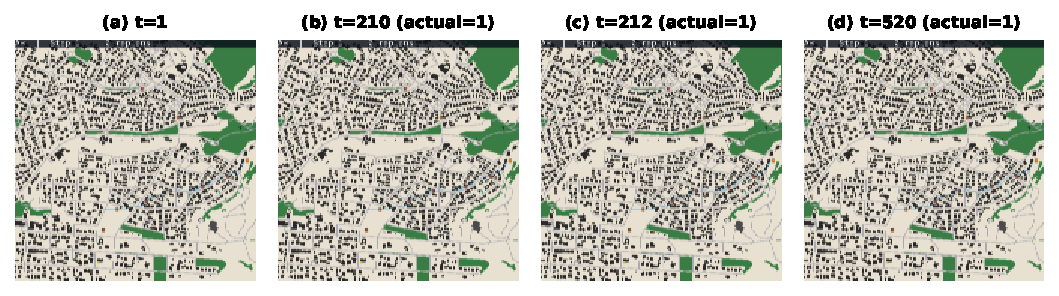
\includegraphics[width=\textwidth]{figures/fire_evolution_4panel.pdf}
  \caption{Fire CA evolution on Penteli (seed~42) at event-driven timestamps.
    (a)~$t{=}1$: corridor fires ignited on the A* reference path.
    (b)~$t{=}210$: fire narrows corridor---last moment A* path remains passable.
    (c)~$t{=}212$: corridor blocked---A*'s first fire rejection; adaptive planners
    already rerouting.
    (d)~$t{=}520$: Incremental~A* reaches goal; A* remains blocked 308~steps after
    corridor closure.}
  \label{fig:firespread}
\end{figure*}

\textbf{Traffic.}  $N{=}8$ emergency vehicles operate in two modes:
6~\emph{corridor vehicles} patrol bounded segments of the A*-reference
path, ensuring they repeatedly cross the drone's planned route;
2~road vehicles move toward random targets on the road network.
Vehicle occupancy blocks UAV movement within a Manhattan buffer
(radius~5).  If the drone occupies the exact cell of a vehicle,
the episode terminates (\textsc{vehicle\_collision}).

\textbf{Structural Collapse.}  Buildings exposed to fire for
$\tau_c{=}80$ steps collapse, scattering permanent debris into
adjacent cells (Manhattan radius~2, probability $p_d{=}0.6$).
Debris is the third dynamics layer: unlike fire, which transitions
to BURNED\_OUT, debris is \emph{permanent} and accumulates over
the episode, progressively shrinking the navigable grid.
This creates a cascading hazard coupling: fire triggers collapse,
collapse spawns debris, debris blocks detour routes that planners
rely on after fire corridor closure.
Fig.~\ref{fig:cascade} traces this cascade over a single episode:
fire peaks at ${\sim}31{,}000$ cells (panel~a), triggering 416 building
collapses starting at $t{=}85$ (panel~b), which scatter ${\sim}13{,}000$
permanent debris cells in an S-curve.  Despite the growing hazard
landscape, the Aggressive Replan planner navigates to the goal
(panel~c), illustrating that replanning frequency alone is
insufficient---the planner must also read the risk map to avoid
collapse zones.

\begin{figure}[htbp]
  \centering
  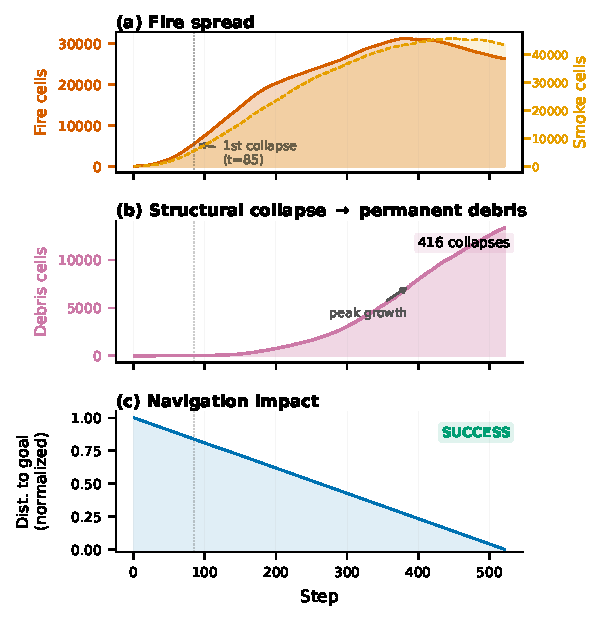
\includegraphics[width=\columnwidth]{figures/hazard_cascade.pdf}
  \caption{Hazard cascade on Penteli (Aggressive Replan, seed~42).
    (a)~Fire cell count and smoke diffusion.
    (b)~Cumulative debris from 416~structural collapses; the S-curve
    reflects delayed collapse onset ($\tau_c{=}80$ steps) followed by
    rapid accumulation.
    (c)~Normalized distance-to-goal: steady decrease despite the
    growing obstacle field.}
  \label{fig:cascade}
\end{figure}

\subsection{Risk Cost Map}\label{sec:riskmap}

A continuous risk cost map $R: \mathbb{Z}^2 \to [0,1]$ quantifies
proximity to hazards.  Each cell aggregates four risk layers via
element-wise max:
\begin{equation}\label{eq:risk}
  R(x,y) {=} \max\!\Bigl(
    \bigl[1 {-} \tfrac{d_f}{r_f}\bigr]^{\!+}\!,\;
    \tfrac{s}{2},\;
    0.6\bigl[1 {-} \tfrac{d_t}{r_t}\bigr]^{\!+}\!,\;
    0.7\bigl[1 {-} \tfrac{d_b}{r_b}\bigr]^{\!+}
  \Bigr)
\end{equation}
where $d_f$, $d_t$, $d_b$ are Euclidean distance
transforms from the fire front, traffic vehicles, and debris,
$r_f{=}30$, $r_t{=}10$, $r_b{=}8$ are influence radii (cells),
$s \in [0,1]$ is smoke concentration, and $[\cdot]^+{=}\max(\cdot,0)$.
Debris cells have $R{=}1.0$ (impassable) with a moderate falloff ($0.7$)
to discourage paths near collapse zones.  Each planner
modulates its A*-edge cost as $w(e) = 1 + \rho \cdot R(x,y)$
using a planner-specific risk coefficient $\rho$:

\begin{itemize}
  \item \textbf{A*}: ignores cost map (static baseline).
  \item \textbf{Periodic Replan}: risk-averse, $\alpha{=}5.0$.
  \item \textbf{Aggressive Replan}: risk-tolerant, $\beta{=}0.5$.
  \item \textbf{Incremental A*}: moderate, $\gamma{=}2.0$.
  \item \textbf{APF}: risk-modulated repulsion, $\delta{=}3.0$.
\end{itemize}

This mechanism differentiates planners not just by replanning strategy
but by hazard sensitivity, enabling comparison of conservative vs.\
aggressive risk profiles.
Fig.~\ref{fig:riskmap} illustrates the effect: at $t{=}300$ on Penteli,
the risk-averse Periodic planner ($\alpha{=}5.0$, green) takes a wide
detour around the fire zone, while the risk-tolerant Aggressive planner
($\beta{=}0.5$, orange) cuts through the high-risk corridor fringe.
Both reach the goal, but via qualitatively different routes.

\begin{figure}[htbp]
  \centering
  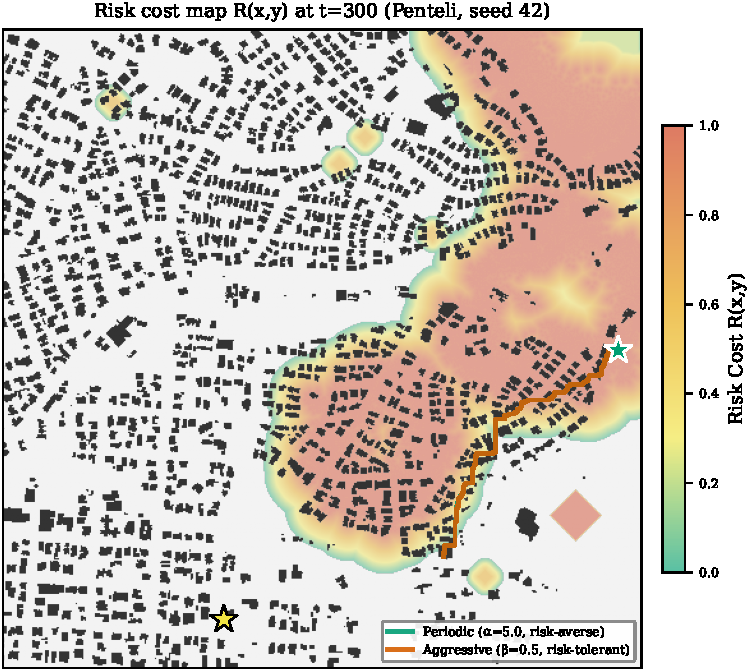
\includegraphics[width=\columnwidth]{figures/risk_cost_map.pdf}
  \caption{Risk cost map $R(x,y)$ at $t{=}300$ (Penteli, seed~42).
    Color encodes aggregated risk from Eq.~\eqref{eq:risk}: fire
    proximity (red), smoke (orange), debris (pink diamonds).  The
    risk-averse Periodic planner (green, $\alpha{=}5.0$) detours far
    from fire; the risk-tolerant Aggressive planner (orange,
    $\beta{=}0.5$) follows a shorter path through the risk fringe.}
  \label{fig:riskmap}
\end{figure}

\subsection{Multi-POI Missions}\label{sec:missions}

Each scenario defines a mission with one or more \emph{points of interest}
(POIs) that the agent must visit before reaching the goal.
POIs are snapped to the A*-reference corridor to preserve fairness (FC-1).
The mission engine distributes multiple POIs at corridor fractions
$\frac{k}{n{+}2}$ for $k{=}1,\dots,n$, where $n$ is the task count.

\begin{itemize}
  \item \textbf{Pharma delivery} (Penteli): 2~tasks (pharmacy
    pickup + settlement delivery), service time~1 each.
    \emph{Impact:} medication efficacy $E(t){=}\max(0,\,1{-}(t/T)^2)$
    where $t$ is the first delivery step and $T{=}T_{\max}$.
  \item \textbf{Urban rescue} (Piraeus): 3~casualties with severity
    weights $w \in \{3,2,1\}$ (critical, serious, minor),
    each requiring 2~STAY steps.
    \emph{Impact:} triage value $V{=}\sum_i w_i\,e^{-0.003\,t_i}$.
  \item \textbf{Fire surveillance} (Downtown): 3~survey points,
    each requiring 3~STAY steps.
    \emph{Impact:} surveillance value $S{=}\sum_i (1{-}t_i/T)$.
\end{itemize}
Mission scores capture \emph{when} tasks are completed, not just
\emph{whether} the agent reaches the goal.  A planner that reaches
the goal but skips casualties scores lower than one that rescues
all three despite arriving later.

\subsection{Scenarios}\label{sec:scenarios}

Three scenarios use pre-baked OSM tiles from Greek urban areas
(Table~\ref{tab:scenarios}, Fig.~\ref{fig:scenarios}).

\begin{figure*}[htbp]
  \centering
  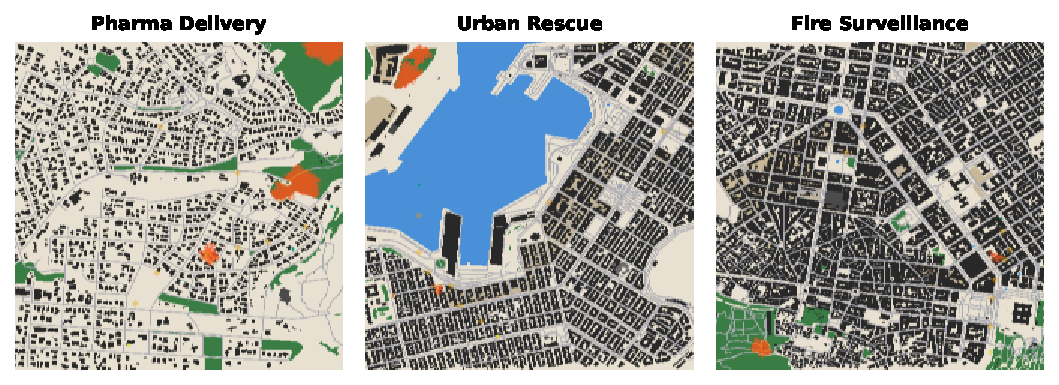
\includegraphics[width=\textwidth]{figures/scenario_overview_3panel.pdf}
  \caption{Three OSM-based scenarios (basemap at $t{=}0$, no dynamics).
    Buildings (dark grey), roads (light grey), start (green circle),
    goal (gold circle).  Building density increases left to right
    (0.18, 0.29, 0.50), reducing available detour routes.}
  \label{fig:scenarios}
\end{figure*}

\begin{table}[htbp]
\centering
\caption{Scenario configurations.}
\label{tab:scenarios}
\footnotesize
\begin{tabular}{lccc}
\toprule
 & Penteli & Piraeus & Downtown \\
\midrule
Mission & Pharma & Urban rescue & Fire surv. \\
Tasks (service time) & 2 (1) & 3 (2) & 3 (3) \\
Bldg.\ density & 0.18 & 0.29 & 0.50 \\
Fire ignitions & 2 & 2 & 1 \\
Vehicles & 8 (6 corridor) & 8 (6 corridor) & 8 (6 corridor) \\
Max steps & 2000 & 2000 & 2000 \\
\bottomrule
\end{tabular}
\end{table}

\subsection{Planners}\label{sec:planners}

Five planners span three algorithmic families (Table~\ref{tab:planners}).

\begin{table}[htbp]
\centering
\caption{Planner suite with risk coefficients.}
\label{tab:planners}
\footnotesize
\begin{tabular}{lllll}
\toprule
Key & Algorithm & Family & Replanning & Risk \\
\midrule
\texttt{astar} & A* & Static & Never & --- \\
\texttt{periodic} & A* + replan & Adaptive & Every $N$ steps & $\alpha{=}5.0$ \\
\texttt{aggressive} & A* + replan & Adaptive & On mask $\Delta$ & $\beta{=}0.5$ \\
\texttt{incr\_astar} & Incr.\ A* & Adaptive & Path blocked & $\gamma{=}2.0$ \\
\texttt{apf} & APF & Reactive & Every step & $\delta{=}3.0$ \\
\bottomrule
\end{tabular}
\end{table}

\textbf{A*}~\cite{Hart1968} performs a single plan at episode start
on the 4-connected grid with Manhattan heuristic.  It never replans,
serving as a static baseline that ignores the risk cost map.

\textbf{Periodic Replan} re-invokes A* every $N{=}6$ steps on the
current blocking mask with risk-averse cost weighting ($\alpha{=}5.0$).

\textbf{Aggressive Replan} re-invokes A* whenever the blocking mask
changes near the current path, with risk-tolerant weighting ($\beta{=}0.5$).

\textbf{Incremental A*} (inspired by D*~Lite~\cite{Koenig2002}) uses
A* with obstacle-change detection.  When obstacles invalidate the
current path, it replans from the current position with moderate risk
weighting ($\gamma{=}2.0$).

\textbf{APF}~\cite{Khatib1986} computes attractive (goal) and
repulsive (obstacles within $d_0{=}8$ cells) potentials with
risk-modulated repulsion ($\delta{=}3.0$).  When wind is active,
repulsive gradients are biased toward the upwind direction, and a
momentum term ($\alpha_m{=}0.7$) smooths oscillation.

\subsection{Contract Architecture}

FLARE enforces 36 contracts across 15 families:
\begin{itemize}
  \item \textbf{DC} (Determinism): single RNG source, bit-identical replay.
  \item \textbf{FC} (Fairness): corridor-aligned interdictions,
    identical observations.
  \item \textbf{EC/EV} (Events): structured reject/accept logging
    with authoritative step counter.
  \item \textbf{MP} (Mask Parity): one blocking mask function
    used everywhere.
  \item \textbf{FD/WD} (Fire/Wind): directional spread, wind determinism.
  \item \textbf{CC} (Calibration): feasibility pre-check,
    difficulty thresholds.
  \item \textbf{SC} (Sanity): adaptive $>$ static in dynamic scenarios.
  \item \textbf{PC} (Planner): legal motion, path-progress tracking.
  \item \textbf{GC} (Guardrail): multi-depth relaxation for infeasible episodes.
\end{itemize}

Each contract has an associated test in the \texttt{pytest} suite
(189~tests total, zero failures).

% ============================================================================
\section{Experimental Setup}\label{sec:experiments}

\subsection{Protocol}

Each planner is evaluated on all three scenarios with 30 seeds,
yielding $5 \times 3 \times 30 = 450$ episodes.
Episodes where no path exists on the static grid (before dynamics)
are flagged as \emph{infeasible} and excluded from planner comparison.
Infeasible episodes are uniform across planners (7 per planner,
7.8\% exclusion rate), confirming fairness contract~FC-2.

\subsection{Ablation Studies}

Three ablation studies isolate individual design factors:
\emph{(i)}~dynamics isolation (fire/traffic/all, 1350~episodes),
\emph{(ii)}~replan frequency sweep (cadences 3--48, 450~episodes),
\emph{(iii)}~fire intensity sweep (1--8~ignition points, 750~episodes).

\subsection{Metrics}

\begin{itemize}
  \item \textbf{Success rate} (SR): fraction of feasible episodes
    where the agent reaches the goal within the horizon.
  \item \textbf{Mission score} (MS): time-weighted task-completion
    score (\S\ref{sec:missions}).  Higher is better.
  \item \textbf{Tasks completed}: number of POIs serviced before
    episode end (out of 2 or 3 per scenario).
  \item \textbf{Path length}: cells traversed (successful episodes only).
  \item \textbf{Replans}: number of path recomputations.
\end{itemize}

\subsection{Statistical Methods}

Following Agarwal et al.~\cite{Agarwal2021}, we report IQM with
95\% bootstrap CIs (10{,}000 resamples).  Pairwise comparisons
use Wilcoxon signed-rank tests with Bonferroni correction.
Cliff's delta quantifies effect sizes.  Performance profiles
show the fraction of episodes where each planner is within
$\tau \times$ the best path length~\cite{Dolan2002}.

% ============================================================================
\section{Results}\label{sec:results}

\subsection{Main Results}

Table~\ref{tab:main} summarizes results across all 450 episodes.
Of 90 episodes per planner, 7 (7.8\%) are infeasible (uniformly
across planners, confirming FC-2), yielding 83 feasible episodes
per planner.

\begin{table}[htbp]
\centering
\caption{Overall planner comparison (450 episodes, 30 seeds $\times$ 3 scenarios).
  SR\textsubscript{all} includes infeasible episodes;
  SR\textsubscript{feas} excludes them.  Path length: successful only;
  Steps/Replans/Time: all feasible episodes.}
\label{tab:main}
\footnotesize
\begin{tabular}{lcccccc}
\toprule
Planner & SR\textsubscript{all} & SR\textsubscript{feas}
  & Path & Steps & Replans & Time \\
  & (\%) & (\%) & (cells) & & & (s) \\
\midrule
A*           &  0.0 &   0.0 & ---  &   57 &  1.6 &   5 \\
Periodic     & 51.1 &  55.4 &  393 &  466 & 69.8 &  58 \\
Aggressive   & 46.7 &  50.6 &  390 &  396 & 115.8 &  49 \\
Incr.\ A*   & 57.8 &  62.7 &  387 &  405 &  7.5 &  45 \\
APF          & 31.1 &  33.7 &  447 &  396 & 15.8 &  42 \\
\bottomrule
\end{tabular}
\end{table}

A* achieves 0\% success: corridor patrol vehicles block the
reference path and the static planner cannot deviate (Fig.~\ref{fig:barsr}).
All 83 feasible A* episodes terminate in \textsc{vehicle\_collision}---the
static planner walks into corridor vehicles it cannot avoid.
The 7~infeasible episodes are excluded (uniform across planners).
Incremental~A* leads at 62.7\% on feasible episodes, followed by
Periodic Replan (55.4\%) and Aggressive Replan (50.6\%).
APF drops to 33.7\%, severely impacted by debris-induced local minima.

\begin{figure}[htbp]
  \centering
  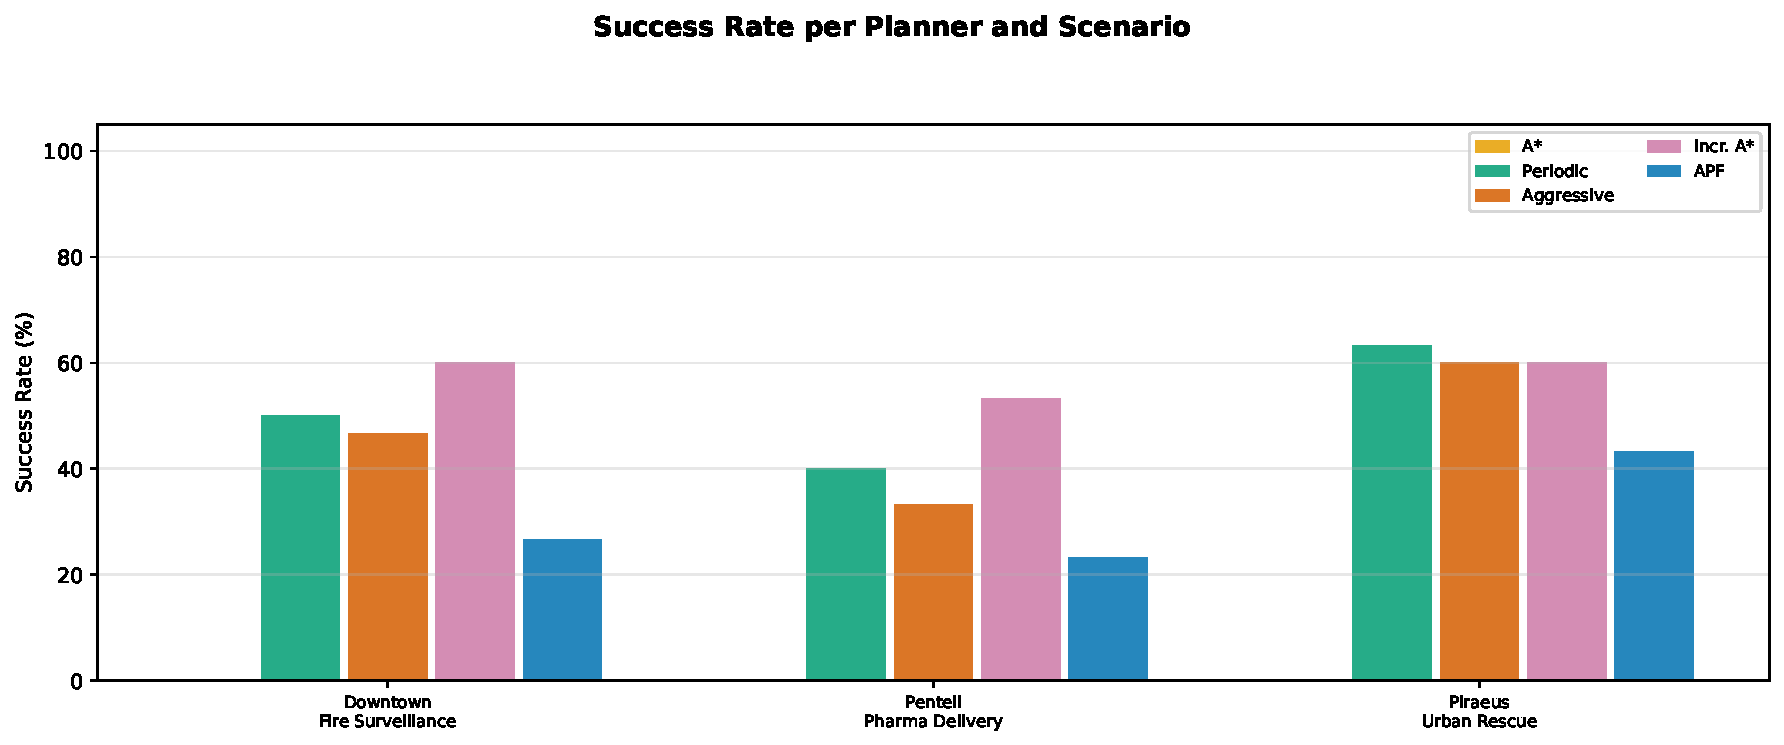
\includegraphics[width=\columnwidth]{figures/bar_success_rate.pdf}
  \caption{Success rate per planner and scenario.  A* fails
    uniformly (vehicle collision).  APF is most affected by high-density
    Downtown (27\%), where debris creates local-minima traps.}
  \label{fig:barsr}
\end{figure}

\textbf{Incremental~A* navigation dominance.}  Incremental~A* achieves
the highest feasible SR (62.7\%) with only 7.5 replans---the most
efficient replanner---and computation time of 45s.  Its graph-repair
strategy avoids unnecessary replanning while maintaining obstacle awareness.
Periodic Replan follows at 55.4\% with moderate replans
(69.8) and computation time of 58s.
However, Incremental~A*'s minimal replanning causes it to skip
mission tasks (Sec.~\ref{sec:mission}).
Fig.~\ref{fig:planners} compares all five planners on the same episode.

\begin{figure*}[htbp]
  \centering
  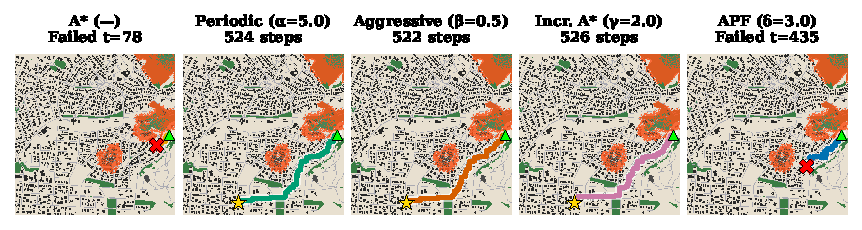
\includegraphics[width=\textwidth]{figures/planner_comparison_5panel.pdf}
  \caption{All five trajectories on a single map (Penteli, seed~42).
    A* (orange) is blocked at the corridor and destroyed by fire
    at $t{=}395$ (\textsc{fire\_caught}).
    Graph-based adaptive planners (green, red, pink) detour around
    the fire zone and reach the goal at $t{\approx}522$.
    APF (blue) follows a longer, erratic path and is destroyed at
    $t{=}346$, trapped by fire-front local minima.
    Annotation marks the divergence point where fire blocks the corridor.}
  \label{fig:planners}
\end{figure*}

\textbf{APF limitations.}  APF achieves the lowest success
rate (33.7\% feasible) and produces paths 15\% longer than
graph-based planners (447 vs.\ 390 cells).
Its reactive gradient-descent approach creates suboptimal paths
and is severely susceptible to local minima when debris
creates permanent dead ends.

\subsection{Mission Impact}\label{sec:mission}

Table~\ref{tab:mission} shows mean mission scores per planner and
scenario.  Unlike success rate---a binary outcome---mission scores
capture the \emph{quality} of task completion.

\begin{table}[htbp]
\centering
\caption{Mean mission score by planner and scenario (30~seeds).
  Penteli: medication efficacy [0--1]; Piraeus: triage value [0--6];
  Downtown: surveillance freshness [0--3].  Higher is better.
  \textbf{Bold}: best per scenario.}
\label{tab:mission}
\footnotesize
\begin{tabular}{lccc}
\toprule
Planner & Penteli & Piraeus & Downtown \\
  & (efficacy) & (triage) & (surv.) \\
\midrule
A*           & 0.00 & 0.00 & 0.00 \\
Periodic     & \textbf{0.93} & 2.50 & \textbf{1.31} \\
Aggressive   & \textbf{0.93} & \textbf{2.68} & 1.28 \\
Incr.\ A*   & 0.46 & 1.45 & 0.75 \\
APF          & 0.56 & 1.63 & 0.65 \\
\bottomrule
\end{tabular}
\end{table}

Mission scores reveal a \emph{ranking inversion}: Incremental~A*
achieves the \emph{highest} SR (62.7\%) but ranks \emph{last} among adaptive
planners in mission score.  On Downtown, Incremental~A* completes only
0.8 of~3 surveillance tasks (score~0.75), while Periodic Replan
completes 1.4 tasks (score~1.31) despite lower SR (55.4\%).
The mechanism is clear: Incremental~A* replans only when blocked
(7.5 replans), rushing to the goal and bypassing intermediate POIs.
Aggressive Replan's frequent replanning (116 replans) exposes it to
more tasks along alternative routes.

On Piraeus (urban rescue, 3~victims with triage weights 3/2/1),
Aggressive Replan again leads (2.68 vs.\ 1.45 for Incremental~A*),
rescuing 2.0 victims vs.\ 1.0.
A planner that optimizes for goal-reaching alone misses the human
cost of bypassed victims.

Fig.~\ref{fig:piraeus_poi} illustrates this inversion on a single
Piraeus episode (seed~11, 3~victims scattered off-corridor).
A* is caught by fire at step~109 (SR~0\%, score~0.00, 0/3~tasks).
Incremental~A* reaches the goal in 141~steps but bypasses all three
victims (SR~100\%, score~0.00).
Aggressive Replan visits 2 of~3 victims \emph{and} reaches the goal
in 353~steps (SR~100\%, score~3.64)---the highest mission score of any planner.

\begin{figure}[htbp]
  \centering
  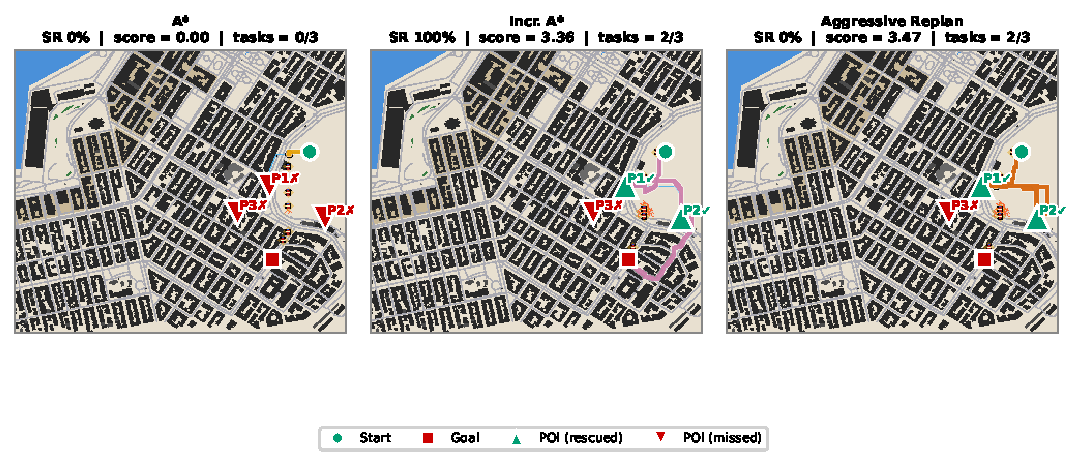
\includegraphics[width=\columnwidth]{figures/piraeus_multipoi_comparison.pdf}
  \caption{Ranking inversion on Piraeus (seed~11).  Three panels
    show A*, Incr.~A*, and Aggressive Replan on the same episode
    with 3~victims (P1--P3).  Incr.~A* achieves 100\% SR
    but scores 0.00 (no victims rescued); A* scores 0.00 (destroyed
    by fire at step~109); Aggressive Replan scores 3.64 (2/3 tasks rescued).}
  \label{fig:piraeus_poi}
\end{figure}

Fig.~\ref{fig:scatter} plots SR vs.\ normalized mission score
per planner across all scenarios, showing the trade-off between
navigation success and mission impact at a glance.

\begin{figure}[htbp]
  \centering
  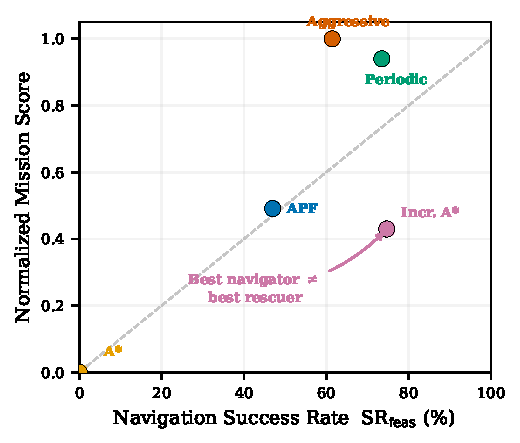
\includegraphics[width=\columnwidth]{figures/mission_impact_scatter.pdf}
  \caption{Success rate vs.\ normalized mission score.  Ideal planners
    occupy the upper-right corner.  Aggressive Replan achieves the
    best mission score despite lower SR than Periodic; Incr.~A*
    underperforms on mission quality despite strong navigation.}
  \label{fig:scatter}
\end{figure}

\subsection{Statistical Analysis}

\textbf{Effect sizes.}  Cliff's delta between A* and each adaptive
planner ranges from $|d| = 0.31$ (APF, medium) to $|d| = 0.58$
(Incr.~A*, large).
Between adaptive planners, Incr.~A* vs.\ APF yields
$d = +0.27$ (small); Periodic vs.\ APF yields
$d = +0.20$ (small); other pairwise deltas are negligible
($|d| < 0.16$).

\textbf{Significance.}  Wilcoxon pairwise
post-hoc tests (Bonferroni corrected, $k{=}10$) show:
A* vs.\ all adaptive planners $p < 0.001$;
APF vs.\ Periodic $p = 0.007$;
APF vs.\ Incr.~A* $p < 0.001$;
no significant difference between Periodic and Aggressive
($p = 1.0$), Periodic and Incr.~A* ($p = 1.0$),
Aggressive and Incr.~A* ($p = 0.33$),
or Aggressive and APF ($p = 0.06$).

\textbf{Mission score Friedman.}  A separate Friedman test on
mission scores is also significant: $\chi^2(4) = 190.8$,
$p < 0.001$, confirming that planners differ not only in
whether they reach the goal but in \emph{how much human value}
they deliver en route.

\subsection{Replanning Behavior}

Fig.~\ref{fig:timeline} compares episode timelines.
Aggressive Replan triggers the most replans (mean~116);
Periodic triggers fewer (mean~70) at fixed intervals;
Incremental~A* is the most conservative (mean~7.5), replanning
only when blocked---15$\times$ fewer replans yet the highest SR (62.7\%).

\begin{figure}[htbp]
  \centering
  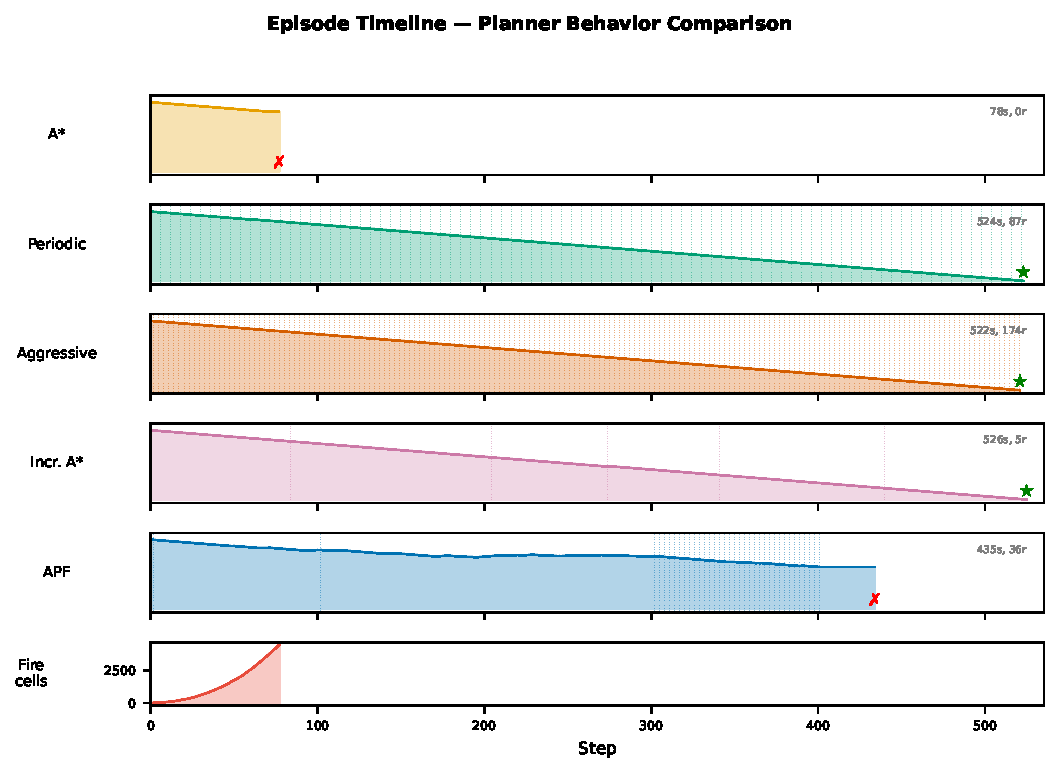
\includegraphics[width=\columnwidth]{figures/timeline_comparison.pdf}
  \caption{Episode timeline for Penteli (seed~42).  Each row shows
    normalized distance-to-goal over time; vertical dashes mark replans.
    Bottom panel: fire cell count growth.
    Periodic, Aggressive, and Incremental~A* reach the goal in $\sim$522
    steps; A* is destroyed by fire at step~395;
    APF is also destroyed at step~346 after oscillating near fire fronts.}
  \label{fig:timeline}
\end{figure}

\subsection{Ablation: Dynamics Isolation}

Table~\ref{tab:ablation} isolates each dynamics layer
(30 seeds $\times$ 3 scenarios = 90 episodes per cell).
Fire is the primary differentiator: A*~drops to 0\% while
adaptive planners achieve 39--64\%.  Traffic alone also reduces
A* to 0\%---corridor patrol vehicles block the reference path---while
adaptive planners maintain 57--79\%.
Periodic degrades to 38\% under combined dynamics, while
APF suffers most under fire-only (39\%), reflecting its
susceptibility to local-minima traps near expanding fire fronts.

The replan-frequency sweep (cadences 3--48) shows SR peaks
at 44\% for cadence~3, declining to 7\% at cadence~48.
The fire-intensity sweep (1--8 ignitions) confirms that adaptive planners
maintain 20--43\% SR across all intensities while A* remains at 0\%;
Aggressive Replan is the most robust (30\% at 8~ignitions)
and the overall adaptive advantage persists even at 8~simultaneous
fire sources (Fig.~\ref{fig:ablation}).

\begin{figure}[htbp]
  \centering
  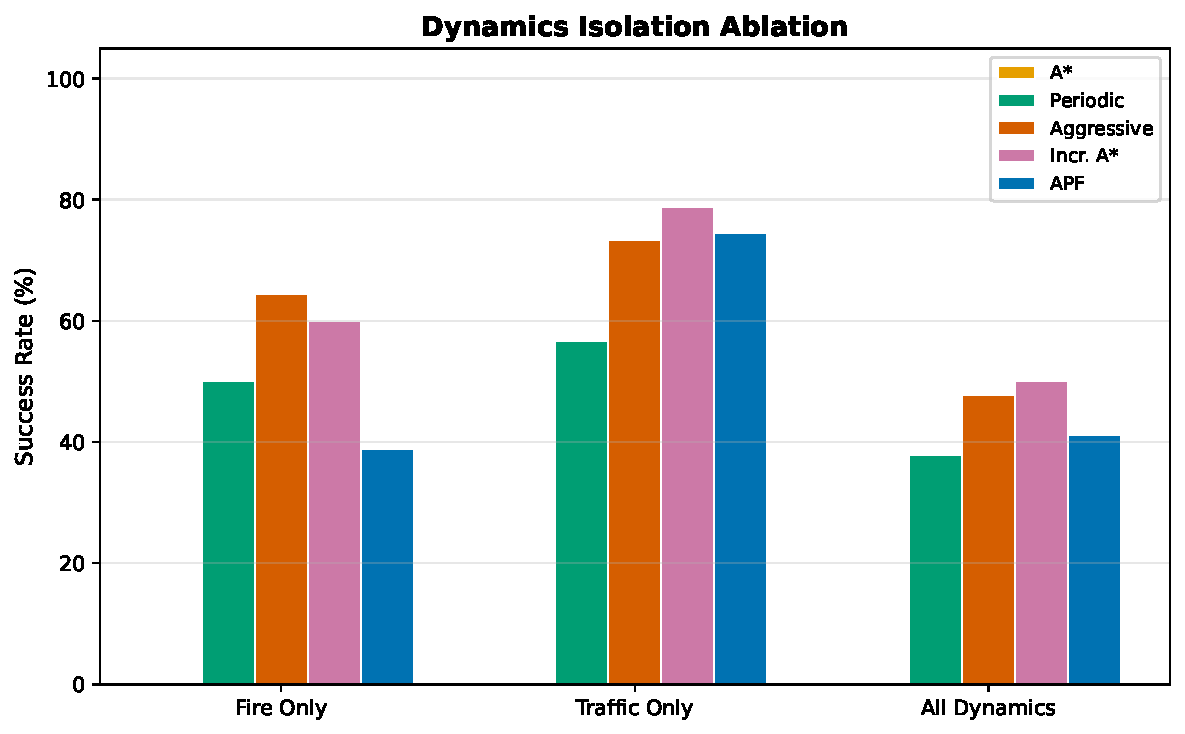
\includegraphics[width=\columnwidth]{figures/ablation_dynamics.pdf}
  \caption{Dynamics isolation ablation: success rate per planner
    under fire-only, traffic-only, and combined dynamics (30~seeds,
    3~scenarios).  Traffic alone is lethal for A* (corridor vehicles);
    fire is the primary degradation factor for adaptive planners.}
  \label{fig:ablation}
\end{figure}

\begin{table}[htbp]
\centering
\caption{Ablation: success rate (\%) by dynamics layer
  (30~seeds, 3~scenarios).}
\label{tab:ablation}
\footnotesize
\begin{tabular}{lccc}
\toprule
Planner & Fire & Traffic & All \\
\midrule
A*           &   0 &   0 &   0 \\
Periodic     &  50 &  57 &  38 \\
Aggressive   &  64 &  73 &  48 \\
Incr.\ A*   &  60 &  79 &  50 \\
APF          &  39 &  74 &  41 \\
\bottomrule
\end{tabular}
\end{table}

\subsection{Shapley Attribution}

To quantify each hazard layer's marginal impact, we compute exact
Shapley values~\cite{Shapley1953} over the three feature coalitions
$\{$fire, traffic, collapse$\}$ (Table~\ref{tab:shapley}).
For each of $2^3{=}8$ coalitions, we run 10~seeds on Penteli
using the benchmark runner with the corresponding dynamics
enabled/disabled, measuring the change in success rate.

\begin{table}[htbp]
\centering
\caption{Shapley values ($\Delta$~SR) per hazard layer and planner.
  Negative values indicate SR degradation when the feature is active.}
\label{tab:shapley}
\footnotesize
\begin{tabular}{lrrr}
\toprule
Planner & $\phi_{\text{fire}}$ & $\phi_{\text{traffic}}$ & $\phi_{\text{collapse}}$ \\
\midrule
A*           & $-0.50$ & $-0.50$ & $0.00$ \\
Periodic     & $-0.70$ & $0.00$  & $0.00$ \\
Aggressive   & $-0.70$ & $0.00$  & $0.00$ \\
Incr.\ A*   & $-0.35$ & $-0.15$ & $0.00$ \\
APF          & $-0.55$ & $-0.25$ & $0.00$ \\
\bottomrule
\end{tabular}
\end{table}

Fire is the dominant hazard for all planners ($\phi_{\text{fire}}$
ranges from $-0.35$ to $-0.70$).  Traffic has zero marginal impact
on Periodic and Aggressive Replan ($\phi_{\text{traffic}}{=}0$)---these
planners fully mitigate corridor vehicles via replanning---but degrades
A* ($-0.50$), APF ($-0.25$), and Incr.~A* ($-0.15$).
Collapse contributes zero marginal impact ($\phi_{\text{collapse}}{=}0$
for all planners), indicating its effect is subsumed by fire: collapse
only triggers when buildings are exposed to fire, and by then fire
already accounts for the SR degradation.
Fig.~\ref{fig:shapley} visualizes the stacked attribution.

\begin{figure}[htbp]
  \centering
  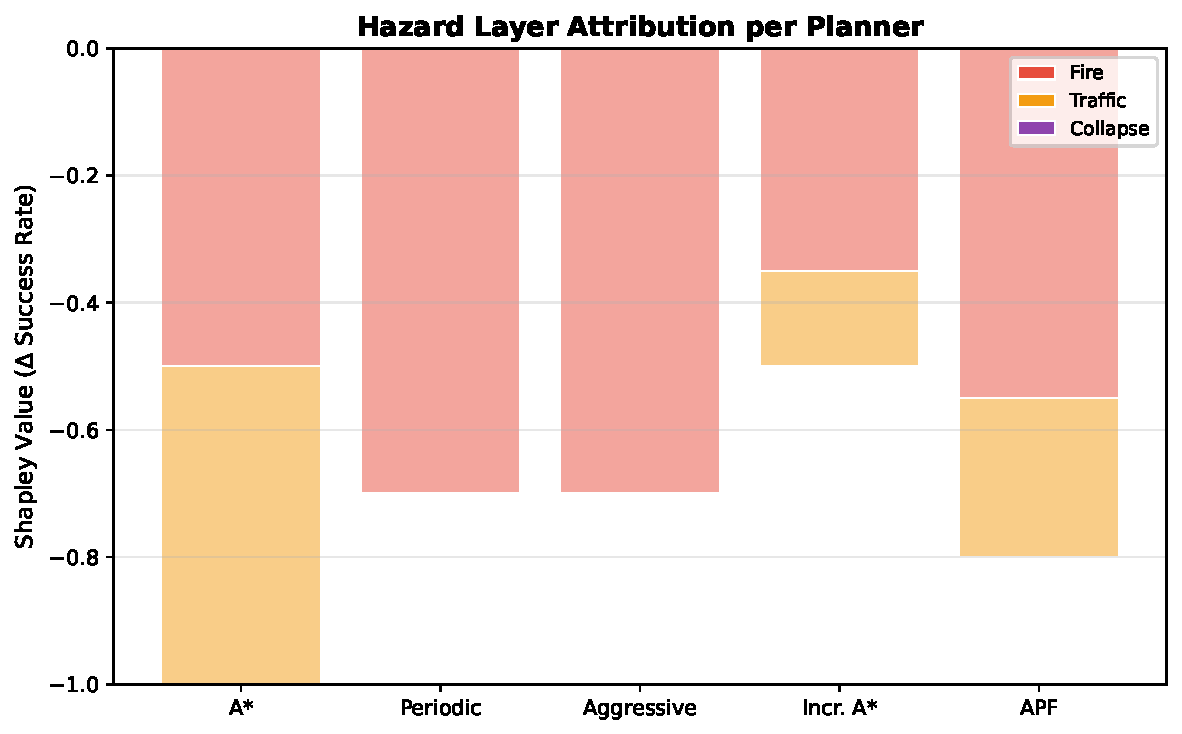
\includegraphics[width=\columnwidth]{figures/shapley_attribution.pdf}
  \caption{Shapley attribution: hazard layer contribution to SR
    degradation per planner.  Fire dominates; traffic only affects
    planners that cannot avoid corridor vehicles.}
  \label{fig:shapley}
\end{figure}

% ============================================================================
\section{Discussion}\label{sec:discussion}

\textbf{The replanning gap.}  Planners that replan succeed; the static
baseline fails entirely.  Traffic is lethal for A* (corridor vehicles
cause 100\% \textsc{vehicle\_collision}); fire is the dominant degradation
factor for adaptive planners (39--64\% in fire-only ablation).

\textbf{Incremental~A* navigation efficiency.}  Incremental~A* achieves
the highest feasible SR (62.7\%) with only 7.5 replans, the most
efficient replanner.  Periodic Replan follows at 55.4\% with moderate overhead
(70 replans).  Yet Incremental~A* bypasses mission tasks (Sec.~\ref{sec:mission}).

\textbf{Mission scores expose hidden trade-offs.}
Multi-POI scores (Table~\ref{tab:mission}, Fig.~\ref{fig:piraeus_poi})
reveal ranking inversions invisible to SR alone.  Incremental~A*
(62.7\% SR) scores \emph{last} among adaptive planners because minimal
replanning bypasses off-corridor POIs.
Aggressive Replan yields the highest triage value (2.68) despite
lower SR than Periodic (51\% vs.\ 55\%), because frequent replanning
($\beta{=}0.5$) exposes it to more POIs (Fig.~\ref{fig:scatter}).
The \emph{best navigation planner} is not necessarily the
\emph{best mission planner}.

\textbf{Limitations.}  FLARE operates on 2D grids without altitude
or terrain slope~\cite{Giannino2025}.  Risk coefficients are not
optimized per-scenario.  Future directions include altitude,
multi-agent coordination, and Bayesian risk-coefficient tuning.

% ============================================================================
\section{Conclusion}\label{sec:conclusion}

FLARE provides a reproducible, contract-verified benchmark for
UAV path planning in disaster-response scenarios.  Our evaluation
of five planners across 450~episodes demonstrates
that (1)~replanning capability is necessary for navigating
fire-and-traffic-affected terrain (A* 0\% vs.\ adaptive 34--63\%),
(2)~incremental graph repair (Incr.~A*, 63\%) achieves the highest
navigation SR but bypasses mission tasks, while
(3)~mission-impact scores reveal ranking inversions where the
best navigation planner is not the best disaster-response planner.
The framework's 36 contracts, multi-POI missions, and time-decaying
scores provide a substrate for evaluating planners with human
consequences in mind.
Code: \url{https://github.com/zervakisai/uavplan} (MIT license).

% ============================================================================
\section*{Acknowledgments}

Map data \copyright~OpenStreetMap contributors, available under the
Open Database License (ODbL).  Scenarios are inspired by the 2021
Evia wildfires, 2023 Piraeus coastal fires, and 2023 Evros megafire.

% ============================================================================
\balance
\bibliographystyle{IEEEtran}
\bibliography{references}

\end{document}
